\documentclass[12pt]{article}

\usepackage{graphicx}
\usepackage{xcolor}
\usepackage{fullpage}

% Variables to easily change filenames:
\newcommand{\firstfile}{Etape1-Neurone.aesl}
\newcommand{\secondfile}{Etape10-Oscillateur.aesl}

\title{Initiation to Neuro-Robotics}
\author{Beno\^{i}t Girard\\\\\textbf{English translation}:\\ Erwan Renaudo}
\date{}

\begin{document}

\maketitle

\tableofcontents


~\\
\textcolor{red}{TODO: EN version of figures}

\section*{Before starting}
\subsection*{About blockly:}

Tables: in blockly, variables are stored in tables by default. When you need only one variable, you have to declare a table of size 1:

\begin{center}
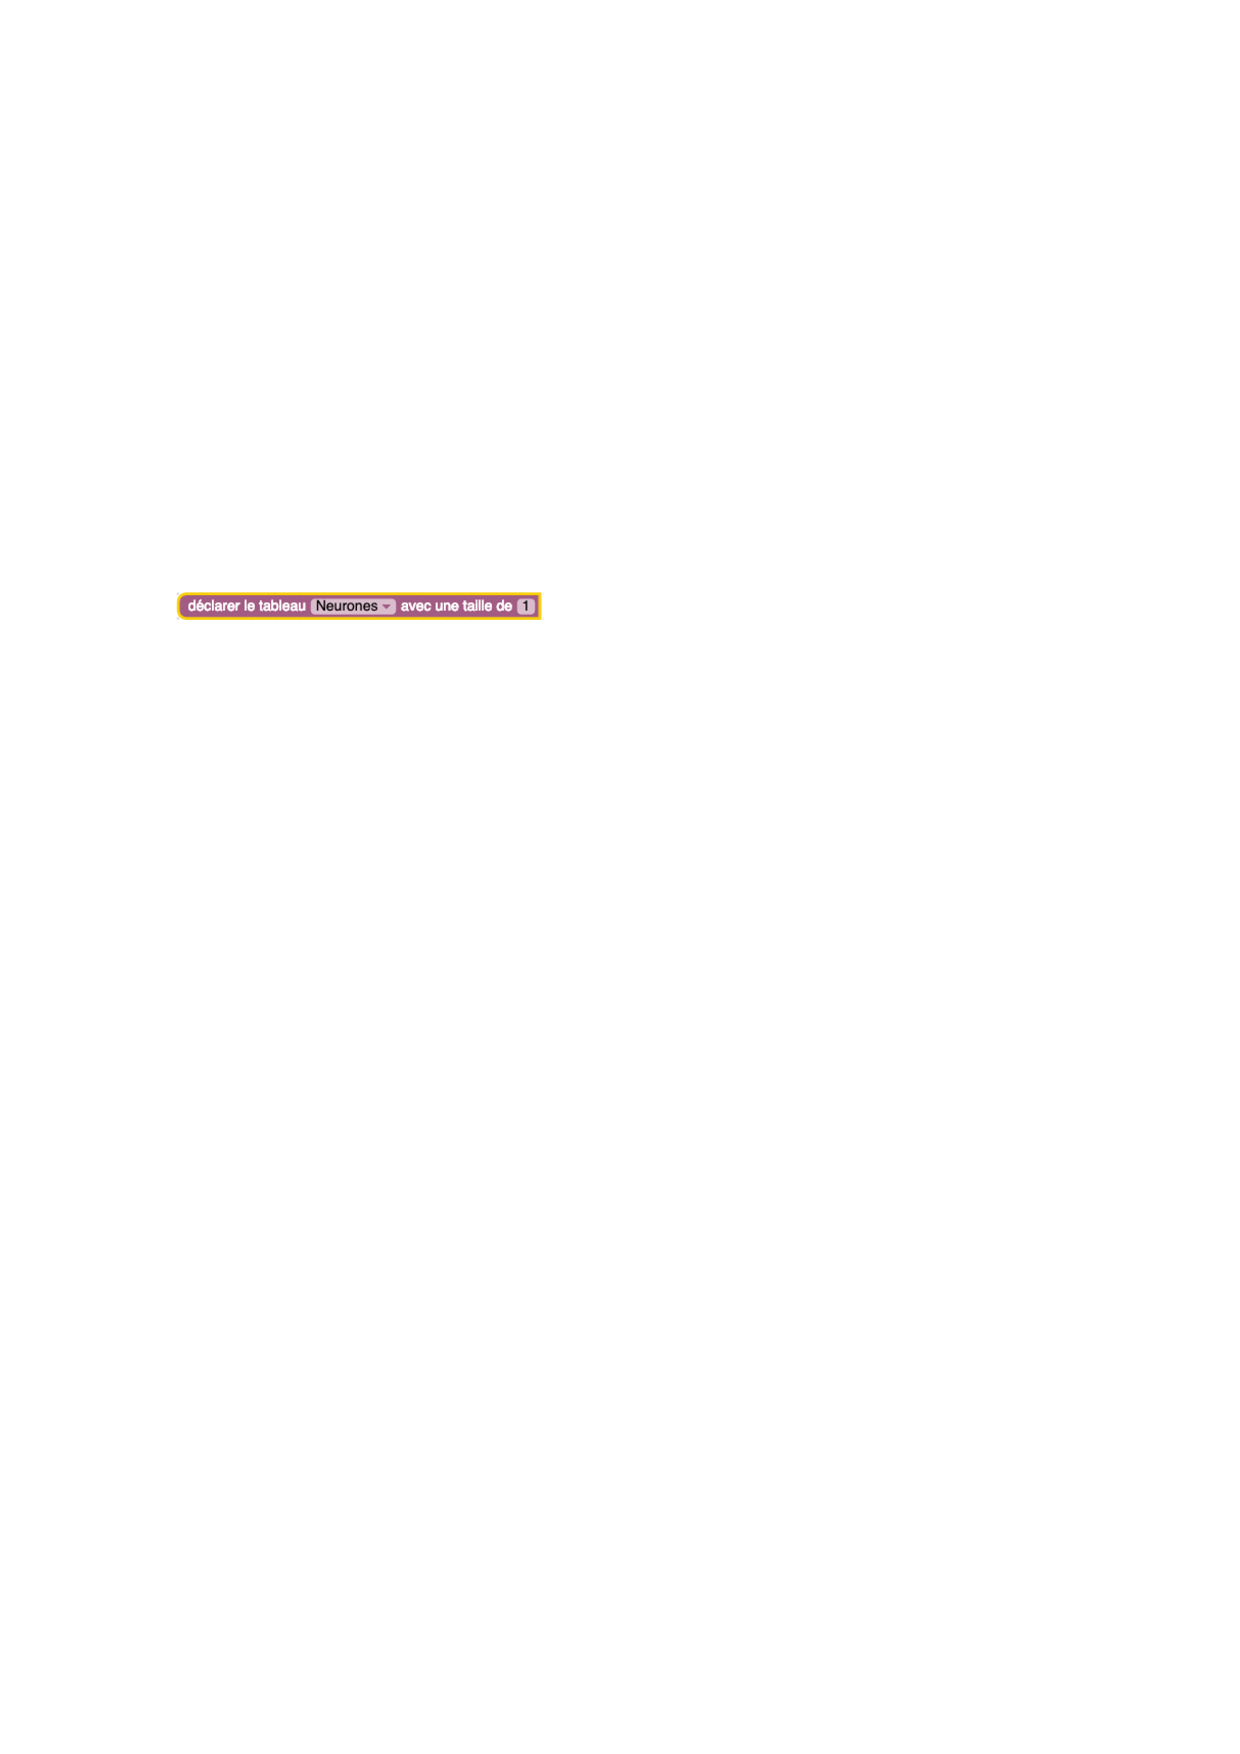
\includegraphics[width=0.5\textwidth]{../DeclarationTableau.pdf}
\end{center}

Variable indexing in tables starts from zero, thus in order to access the first value, you should write:

\begin{center}

\includegraphics[width=0.3\textwidth]{../AccesTableau.pdf}
\end{center}

And for a table of size 4:

\begin{center}
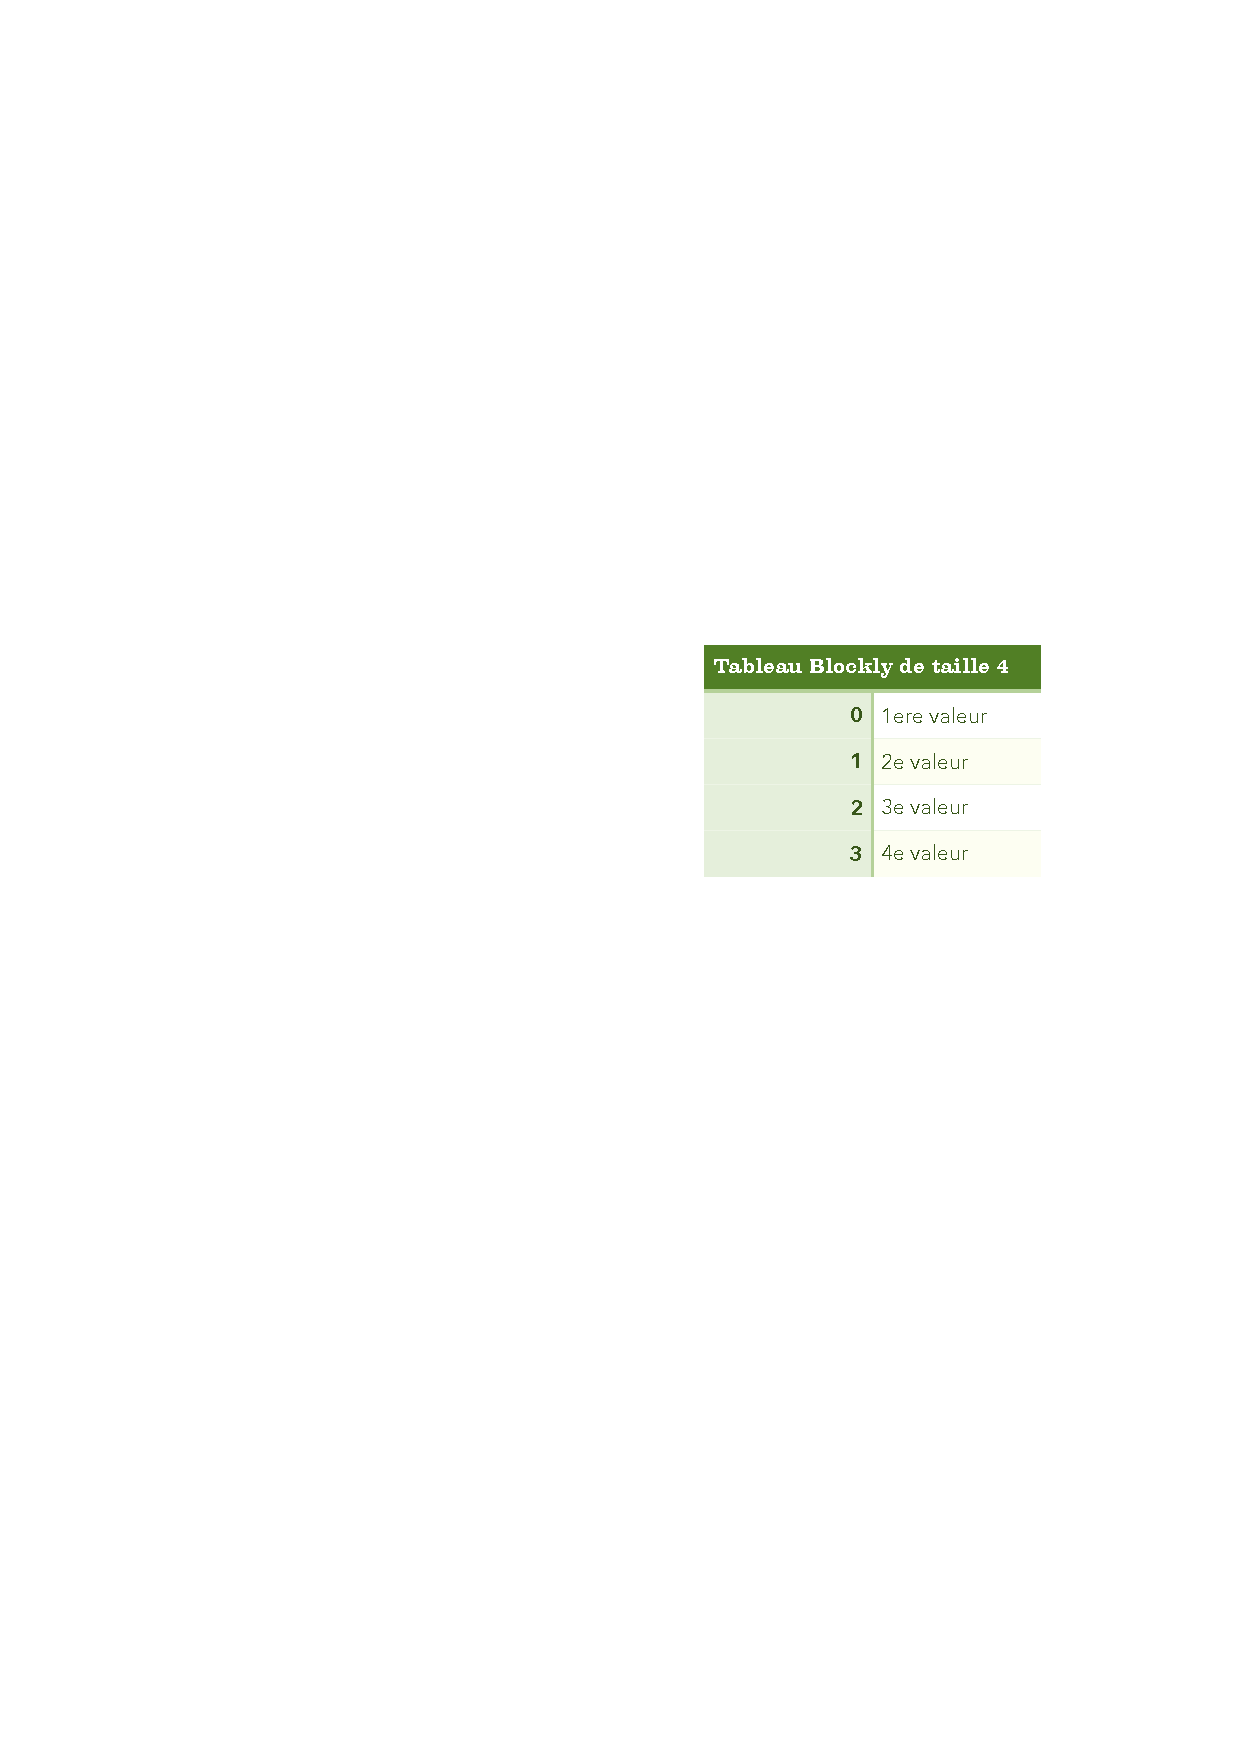
\includegraphics[width=0.3\textwidth]{../StructureTableau.pdf}
\end{center}

\subsection*{About Thymio II}
\begin{itemize}
    \item The distance sensors range from 0 (no visible obstacle) to more than 3000 (when an obstacle is very close).
    \item Motor commands go from -500 (backwards full speed) to 500 (forward full speed).
    \item Orange LEDs values range from 0 (off) to 32 (max brightness).
\end{itemize}

In order to have consistent values in our neural networks, sensor values must be divided by 6 (to range from 0 to 500), and when using a LED to display and activity, this activity must be divided by 16 (to range from 0 to 31).

\begin{center}
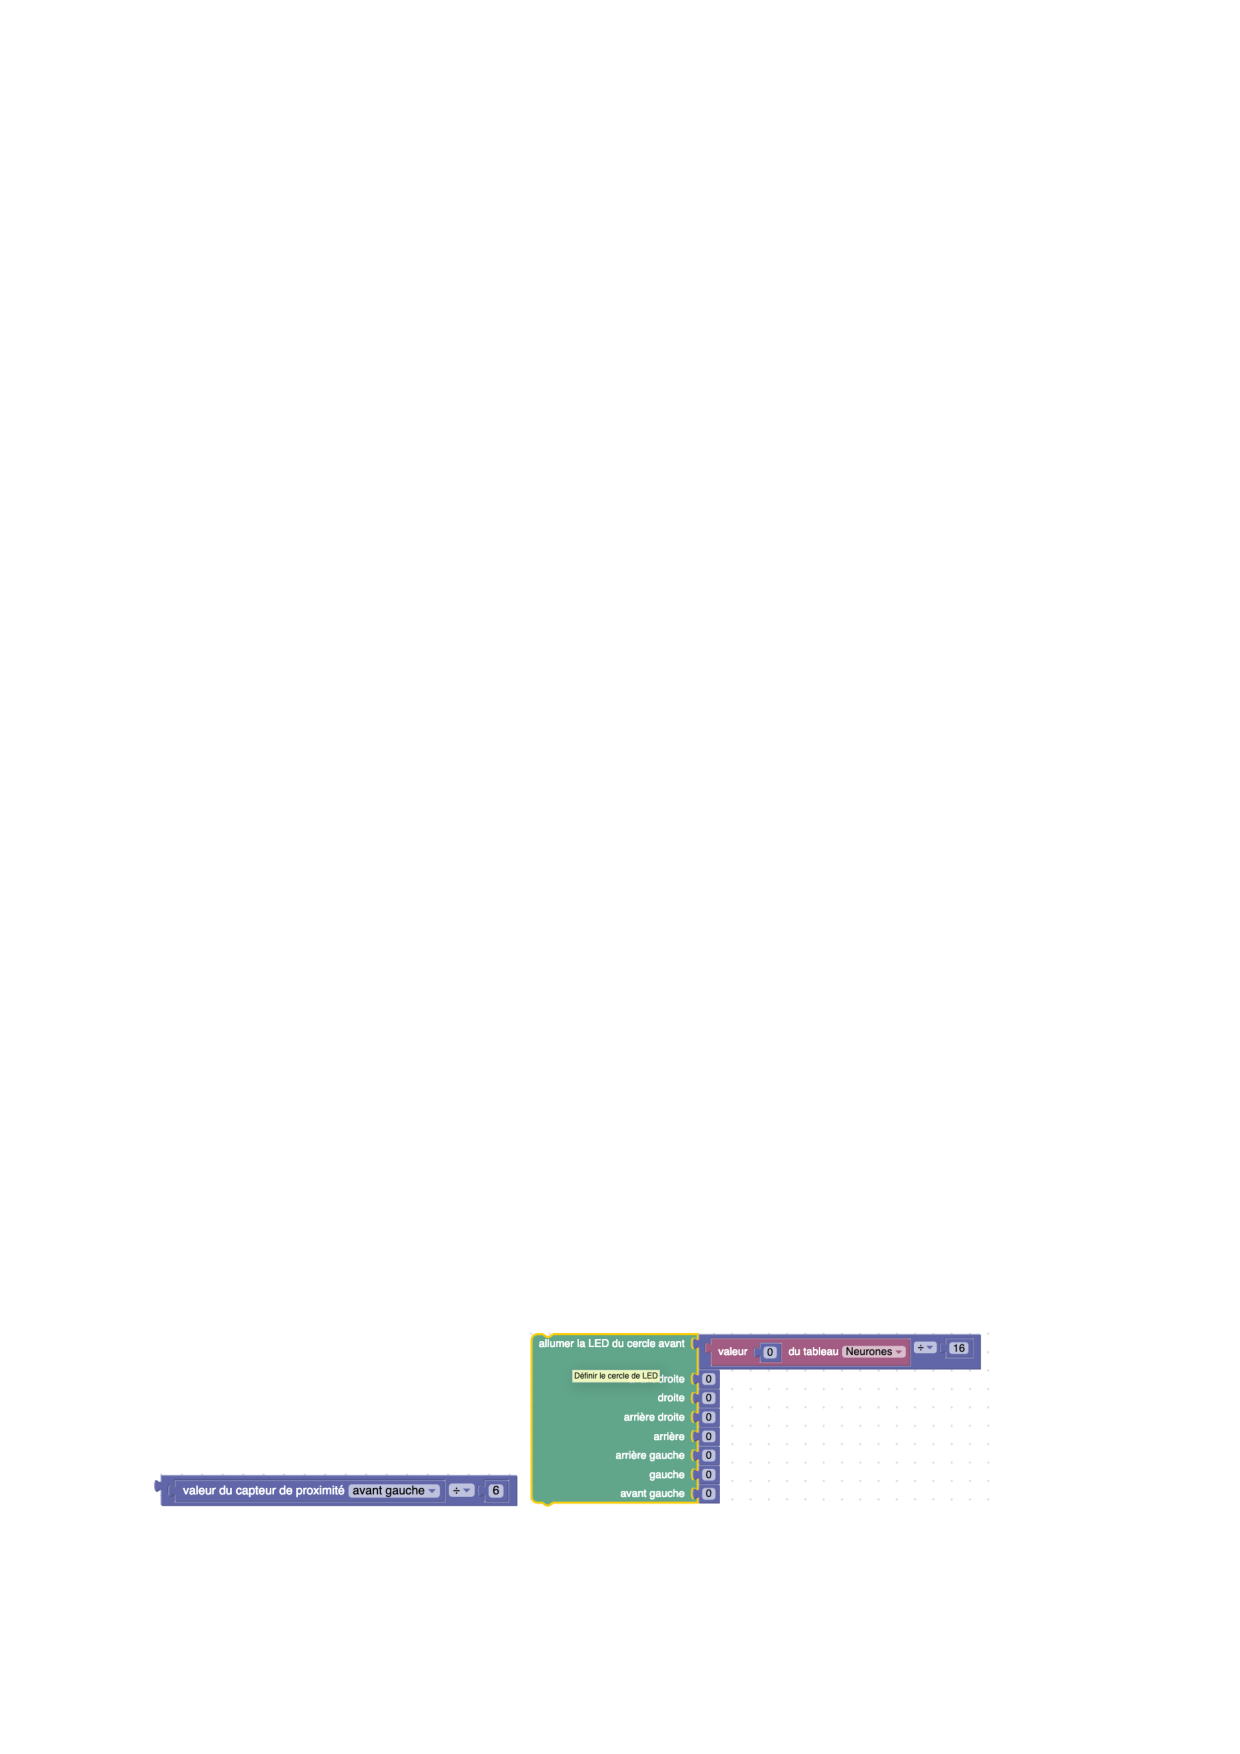
\includegraphics[width=\textwidth]{../Normalisation.pdf}
\end{center}

\section{Programing the first neuron}

The simple artificial neuron model that we will use sums up the input values, constraints them between a minimal (0) and a maximal value (chosen as 500, like the maximal value of motors) and send them to the next neuron.

\begin{center}
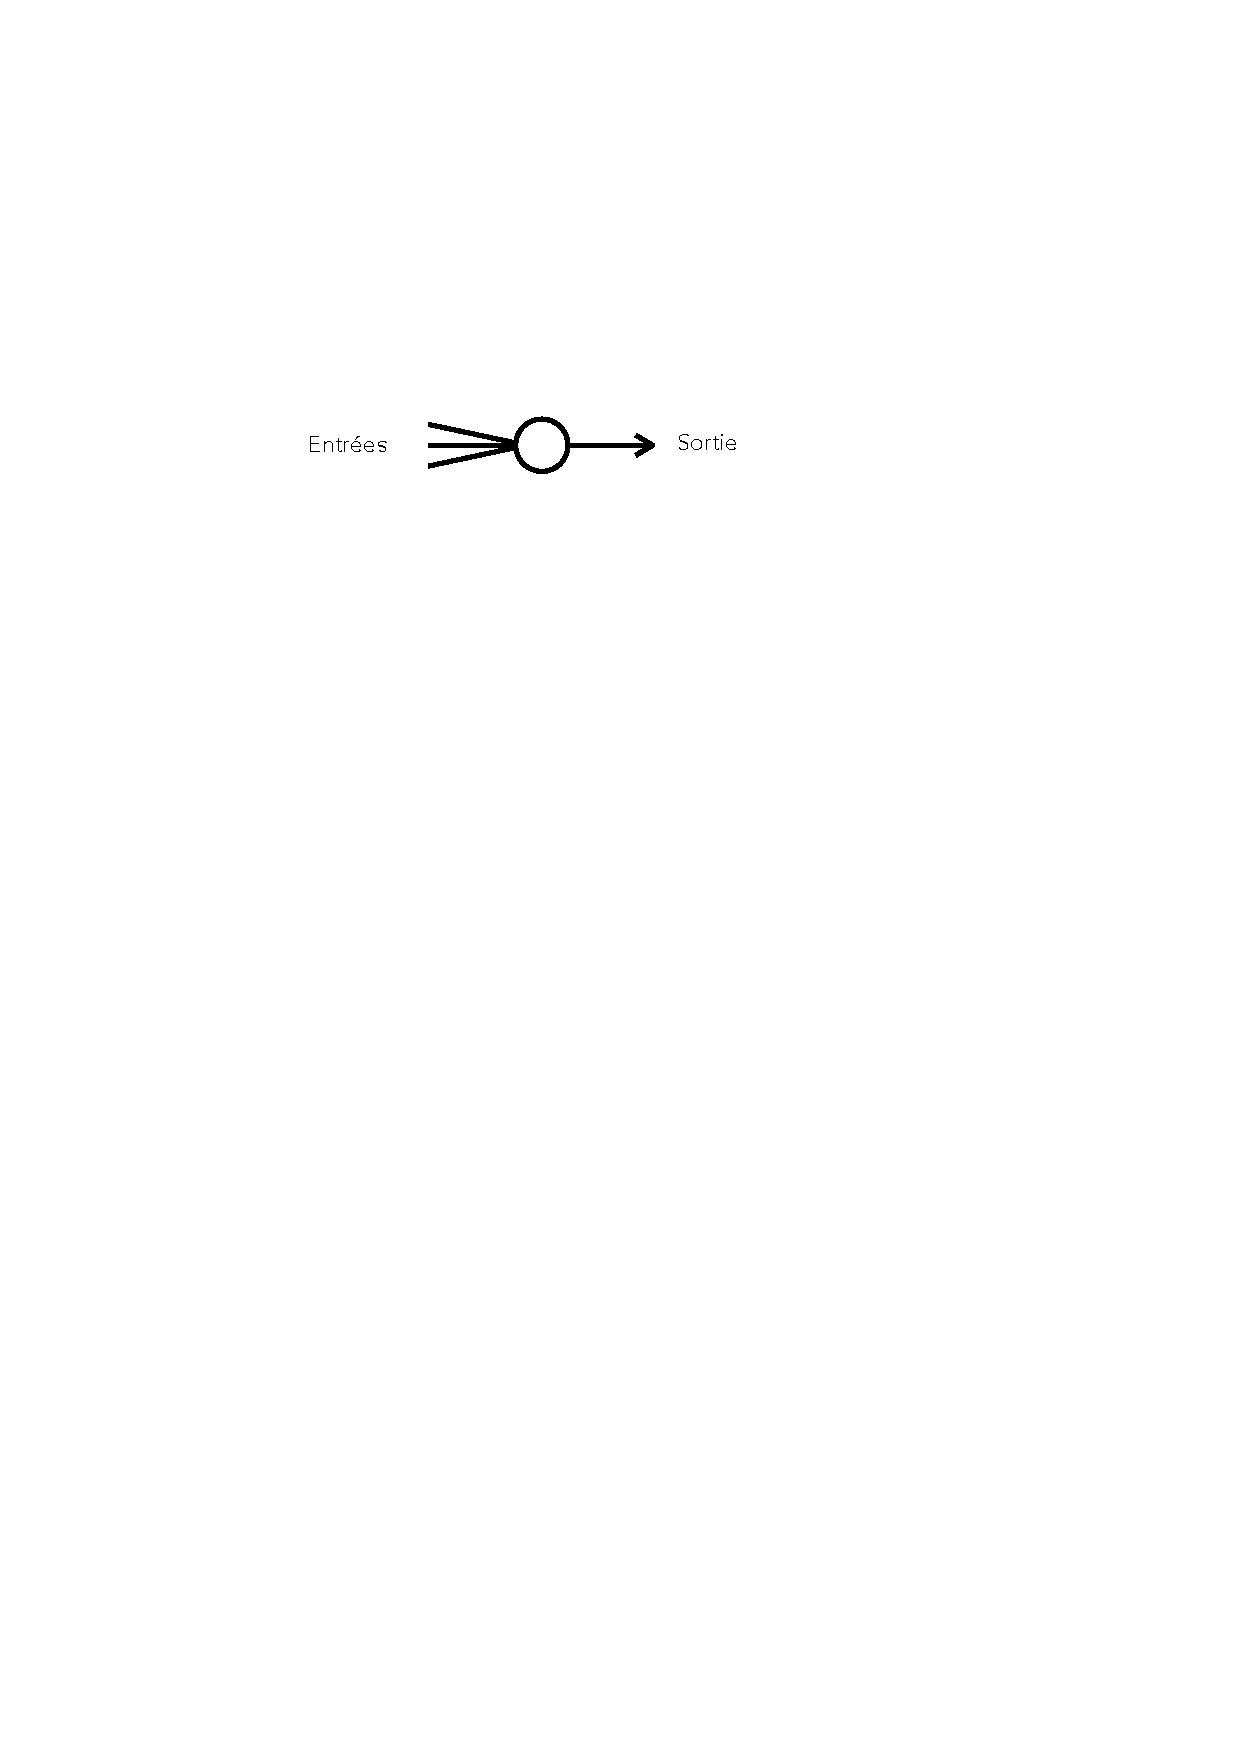
\includegraphics[width=0.5\textwidth]{../SchemaNeuroneArtificiel.pdf}
\end{center}

The output value can be either positive ($+$) or negative ($-$).

\paragraph{Step 1:} Load the file \firstfile, it contains one neuron and a display of its activity. The program should look like that:

\begin{center}
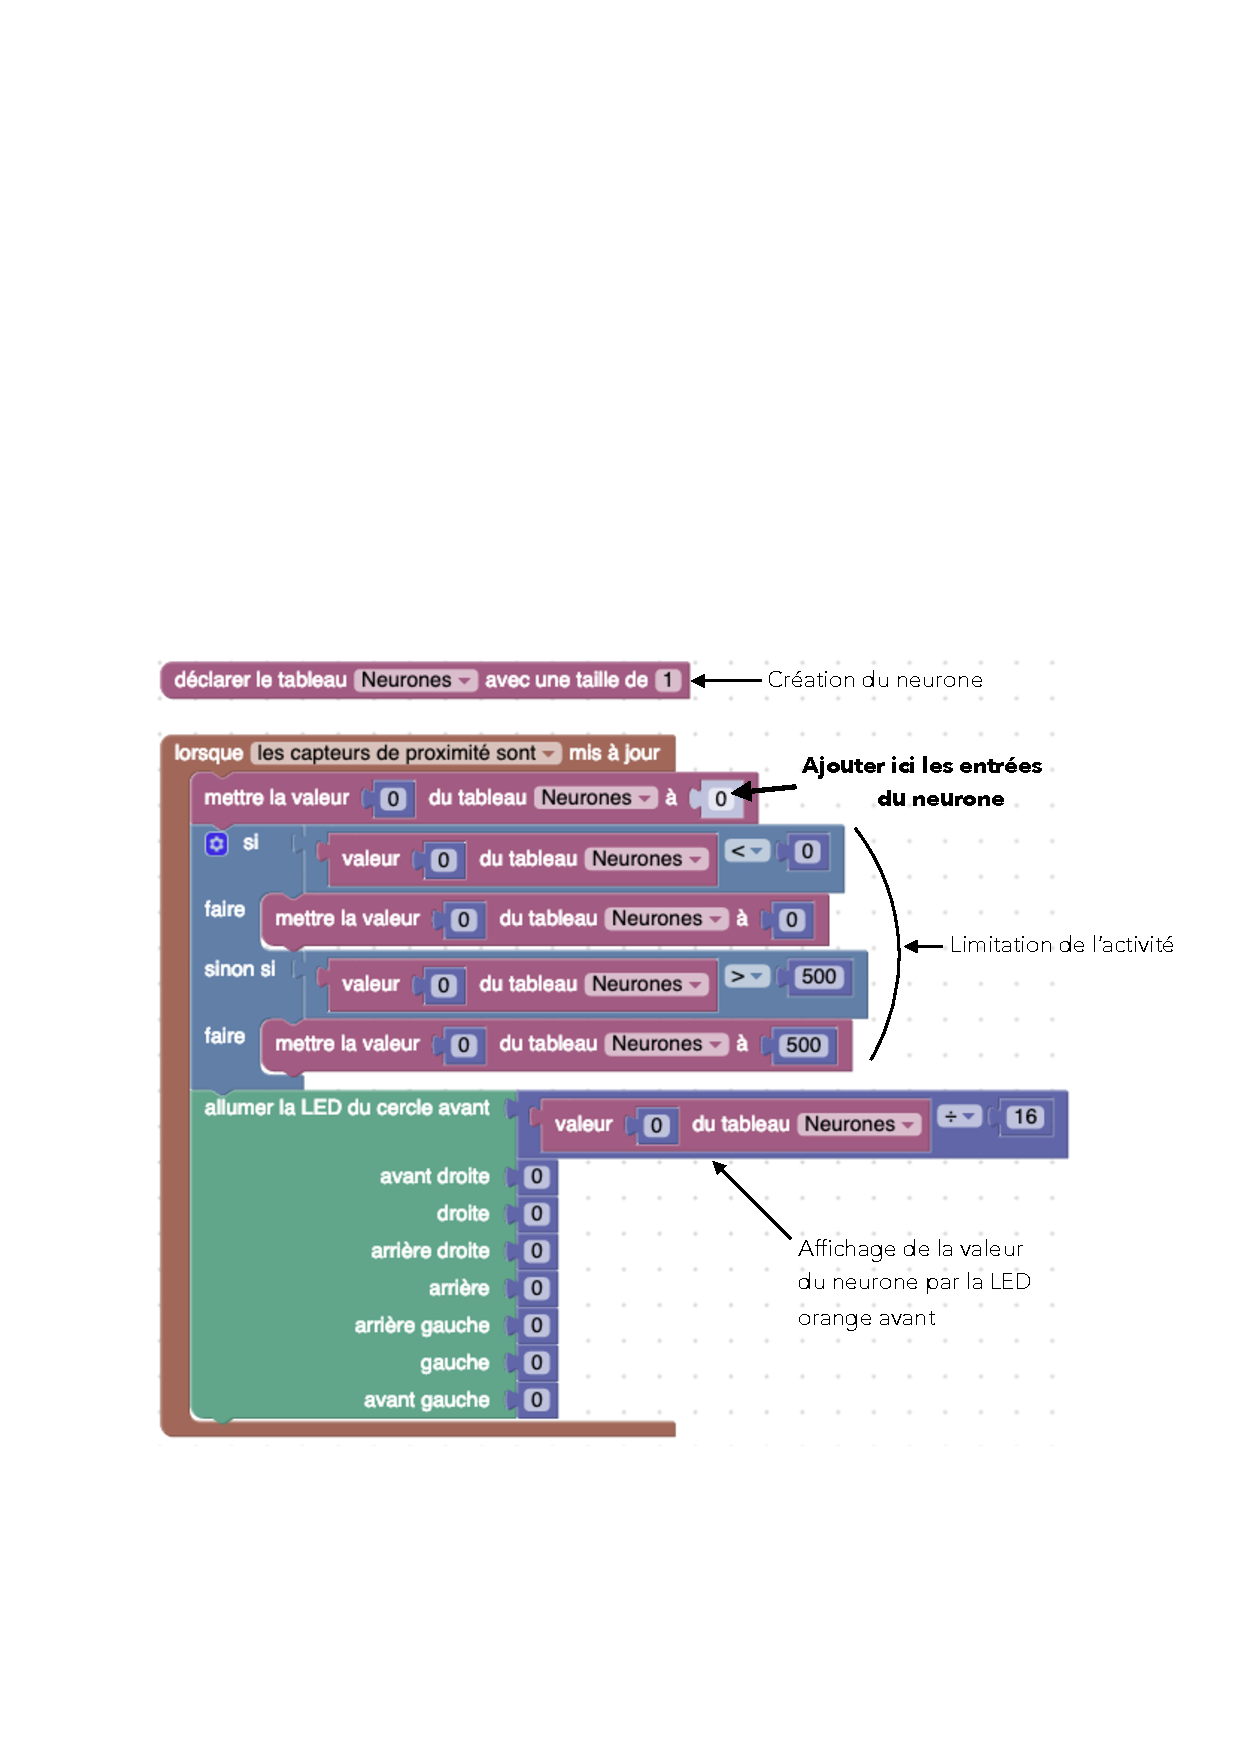
\includegraphics[width=\textwidth]{../ProgrammeEtape1.pdf}
\end{center}

~\\
\begin{center}
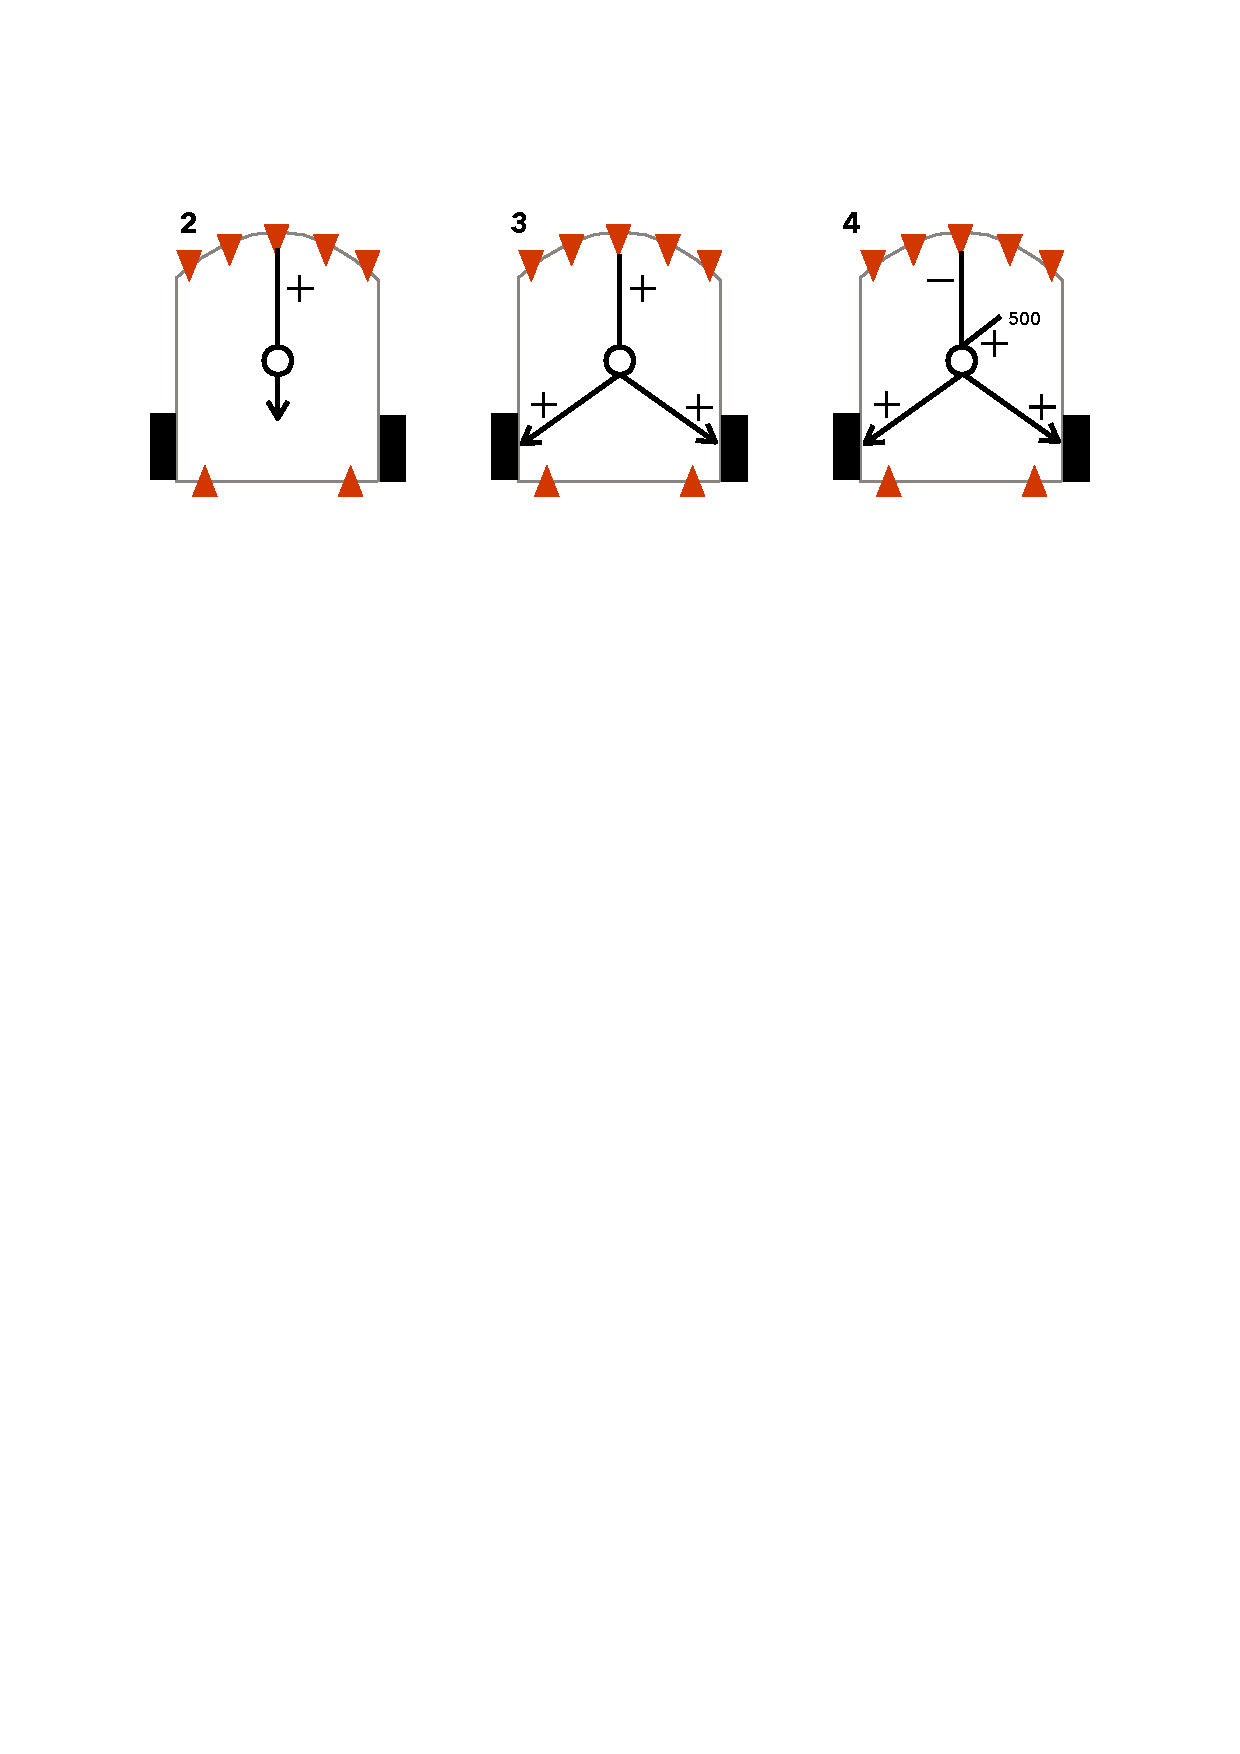
\includegraphics[width=\textwidth]{../Etapes2-4.pdf}
\end{center}

\paragraph{Step 2:} Add a sensor input to this neuron, e.g. using the value of a proximity sensor.

\paragraph{Step 3:} Send its output to motors: given the sensor value, the robot forward speed changes from slow to fast. Our robot has its first (tiny) brain! For now, it's not very clever, it charges at obstacles...

\paragraph{Step 4:} We actually want the robot to always move until there is an obstacle: we add to our neuron a positive input of value 500 and substract the sensor value, then output the result to the motors.

\section{Two neurons}

If we add a second neuron, we will be able to have different activity on each motor, thus not only move in a straight line but also turn.

\begin{center}
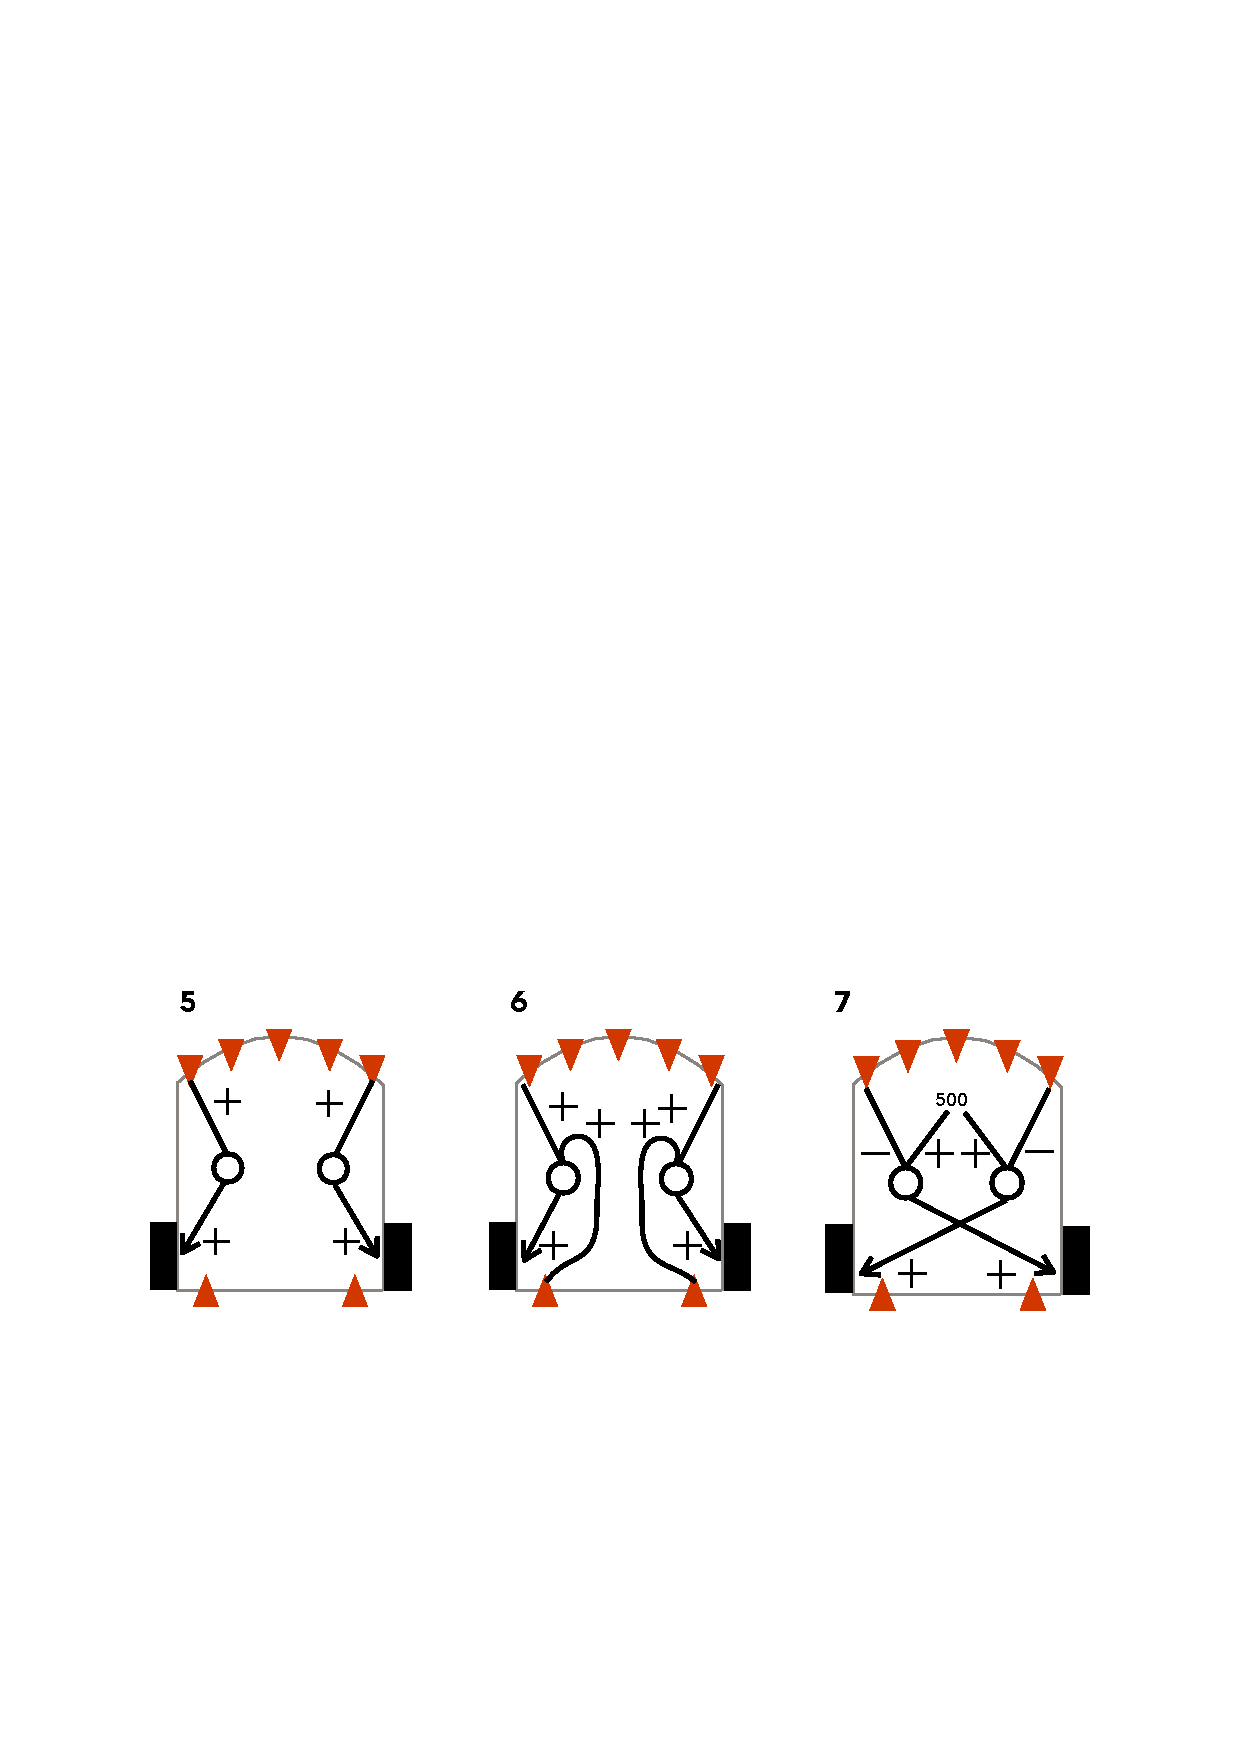
\includegraphics[width=\textwidth]{../Etapes5-7.pdf}
\end{center}

\paragraph{Step 5:} Add a second neuron, connect the neuron 0 input to the front-left sensor nd its output to the left motor. Do the sale thing for neuron 1 with the front-right sensor and the right motor. How does the robot behave if you bring your hand close to it? If you place the robot in a corridor?

\paragraph{Step 6:} Add to your neurons input the back sensors values: the robot moves forward when you try to push it. You can actually make it chase the step 3 robot !

\paragraph{Step 7:} What happens if you stimulate each neuron with a fixed input of value 500 and substract the sensor value, like in step 4? And if you cross-connect neurons to motors (the neuron that gets the left sensor values outputs its value to right motor, and vice versa)?

\section{Internal state with neurons: a memory}

The robot from step 6 goes forward when you put your hand behind to "push it" but stops when you remove your hand. If it had a memory, it could remember it has been pushed and continue moving forward until it encounters an obstacle!

\begin{center}
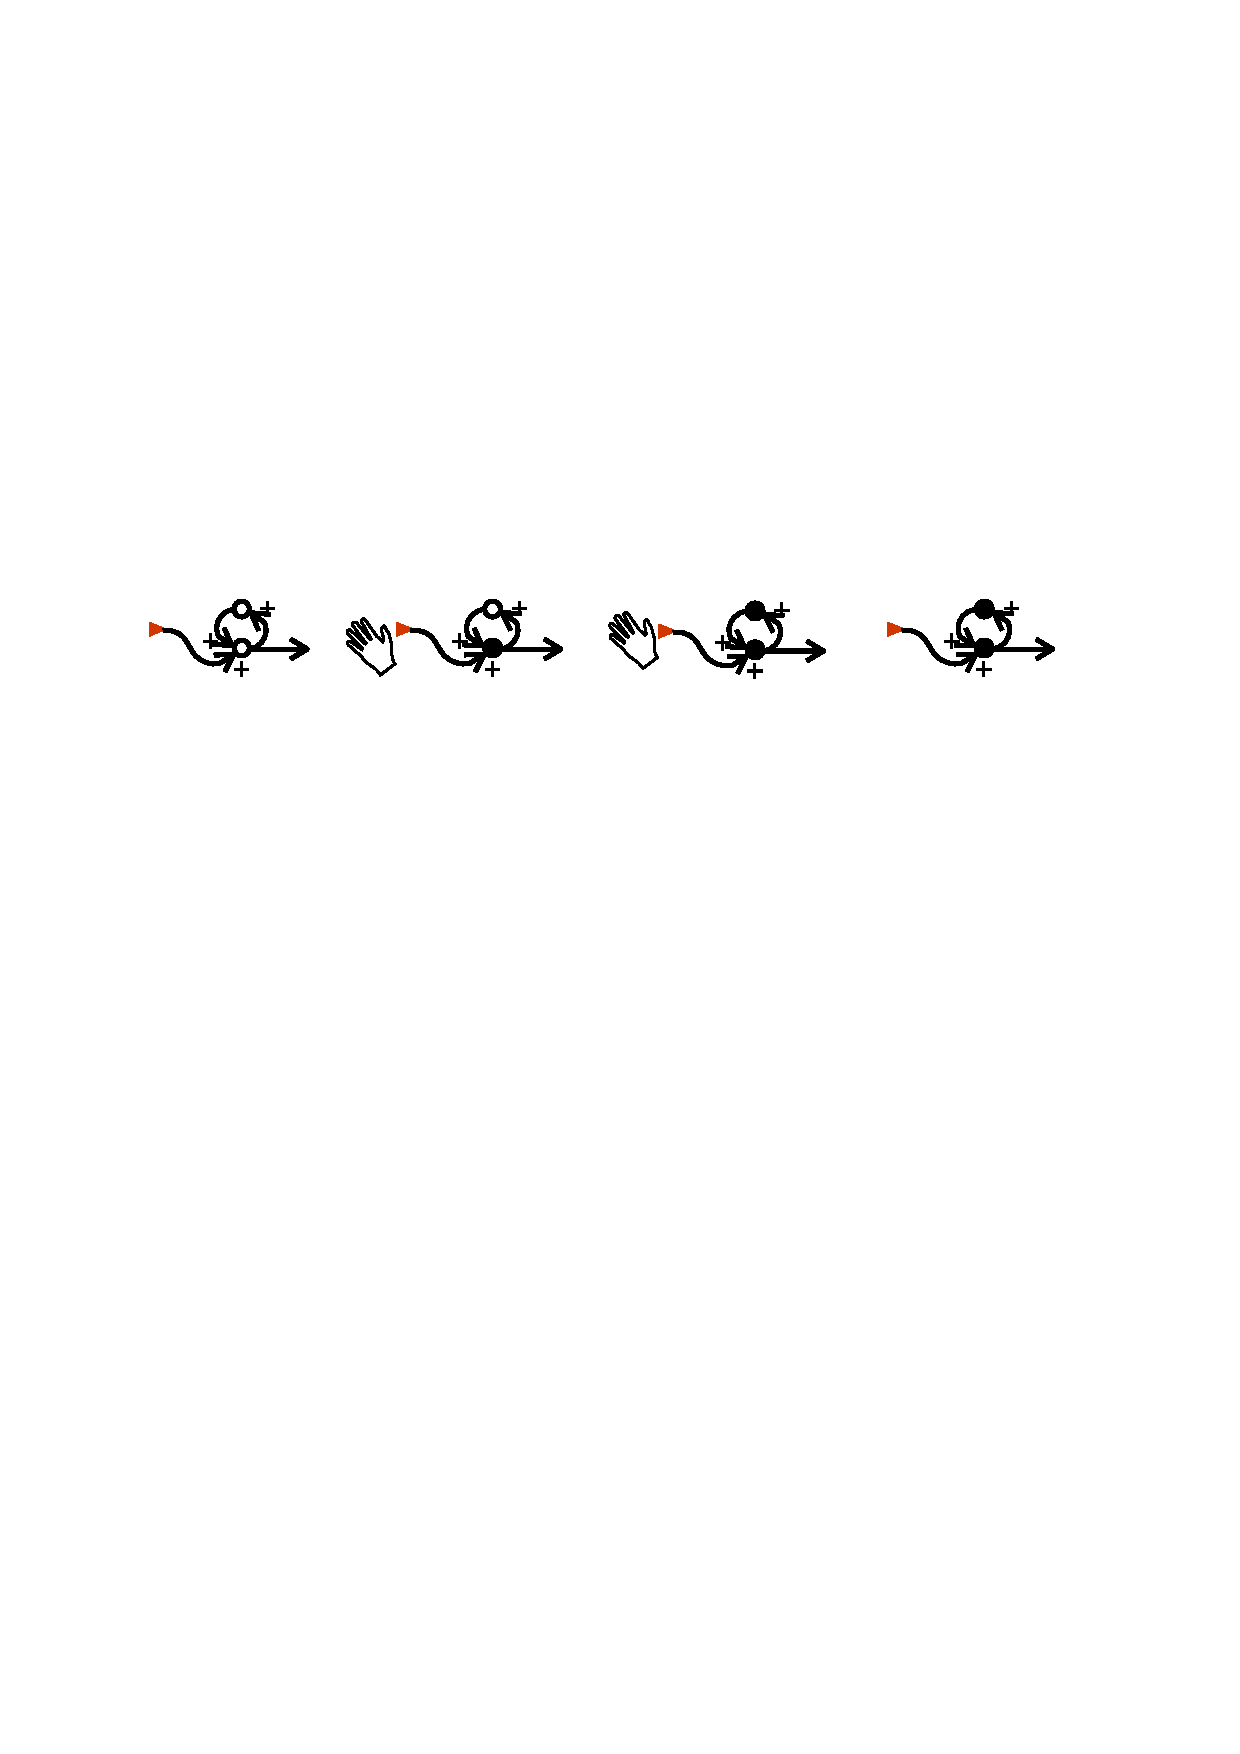
\includegraphics[width=\textwidth]{../Memoire.pdf}
\end{center}


A simple memory can be done by connecting two excitatory neurons in a loop: the first neuron is excited by the proximity of the hand,, it then activate the second neuron, which then activate the first one and so on. Now, when we remove the hand, the excitation loop allows the two neurons to keep exciting each other!

\begin{center}
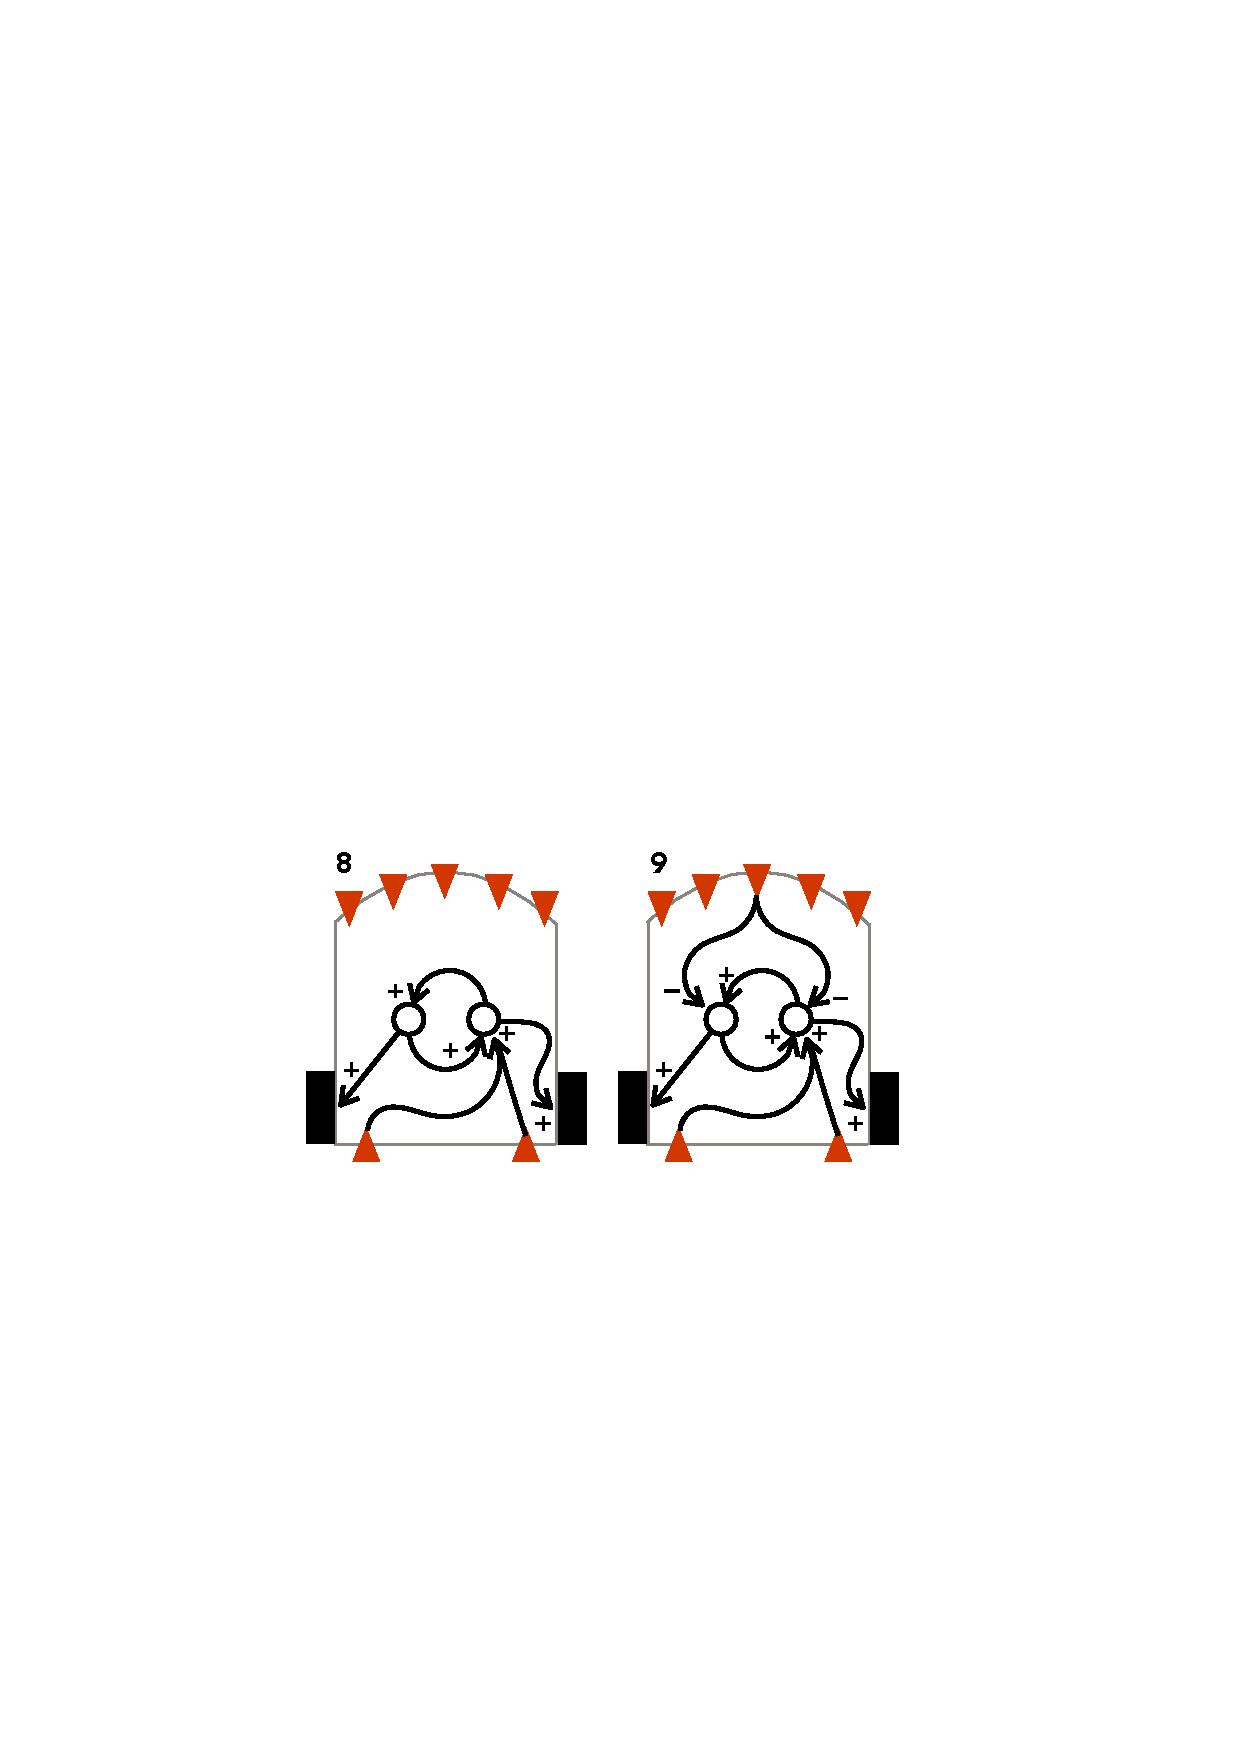
\includegraphics[width=0.66\textwidth]{../Etapes8-9.pdf}
\end{center}

\paragraph{Step 8:} Program the robot such that it moves forward when pushed and keep going when the hand is removed.

\paragraph{Step 9:} Add an inhibition from the front sensor that deactivate the memory when an obstacle is seen in from of the robot.

Robots from steps 1--7 where \emph{reactive}, i.e. they just react to changes in their environment. This new version of the robot has now its own internal activity thank to the memory loop.

\section{Internal state with neurons: oscillations}

Our memory, while activated, has a fixed value over time. If we add a substraction in the loop, we can get a long-lasting activity that varies over time.

\begin{center}
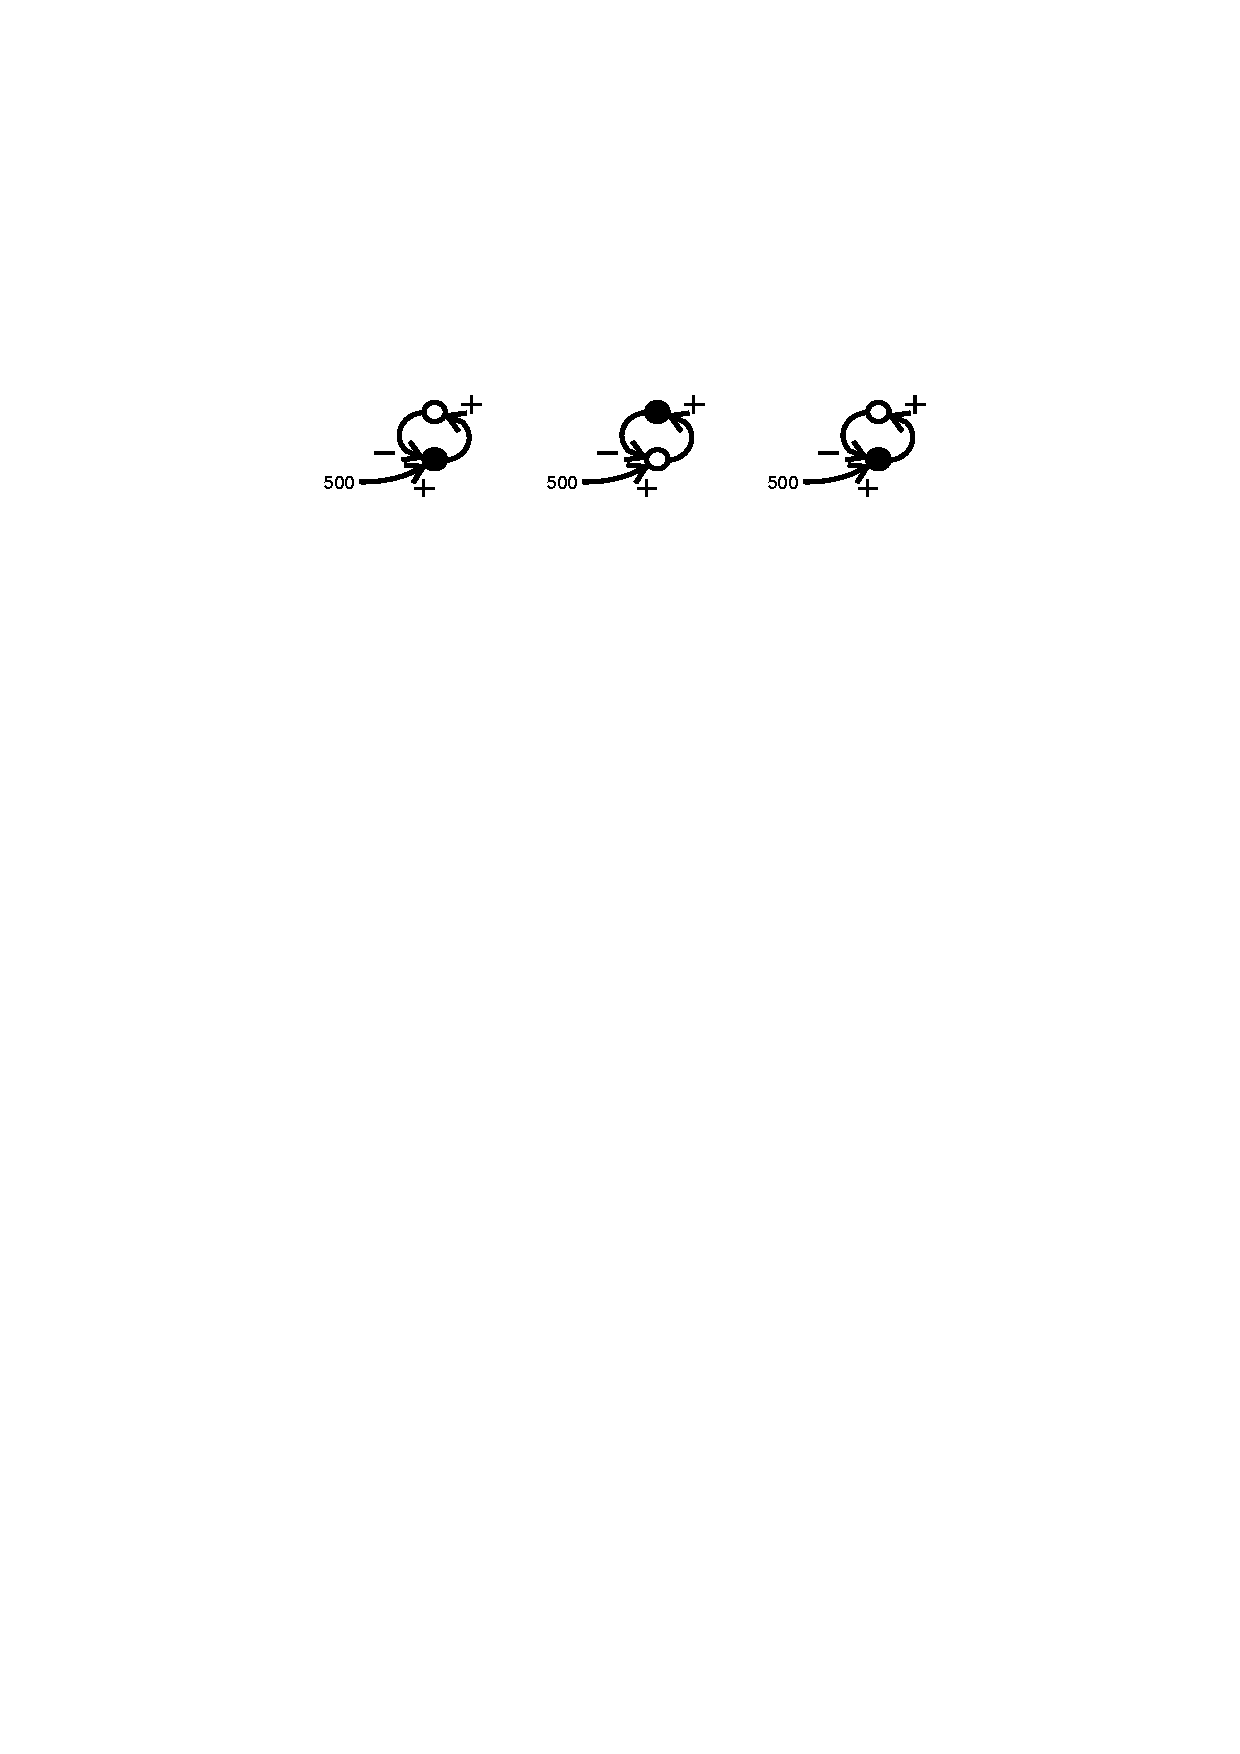
\includegraphics[width=0.66\textwidth]{../Oscillations.pdf}
\end{center}


To make this network work, there is a technical difficulty to overcome: in a real neural network, all activities are computed at the same time from the past activities. In our case, we first compute the value of the first neuron \emph{then} the second. Thus, the second calculation will use the \emph{new} value for the first neuron -- that we just computed -- rather than the past one. This prevent our oscillator to work!

The solution consists in creating a new variable, "PreviousValue" to store the old value of neuron 0, compute the new value of neuron 0 and then compute the new value of neuron 1 using "PreviousValue".

\paragraph{Step 10:} Load file \secondfile, it already contains this new value and the value copy operation. You just need to fill in the connections to observe the oscillations on the orange LEDs.

\begin{center}
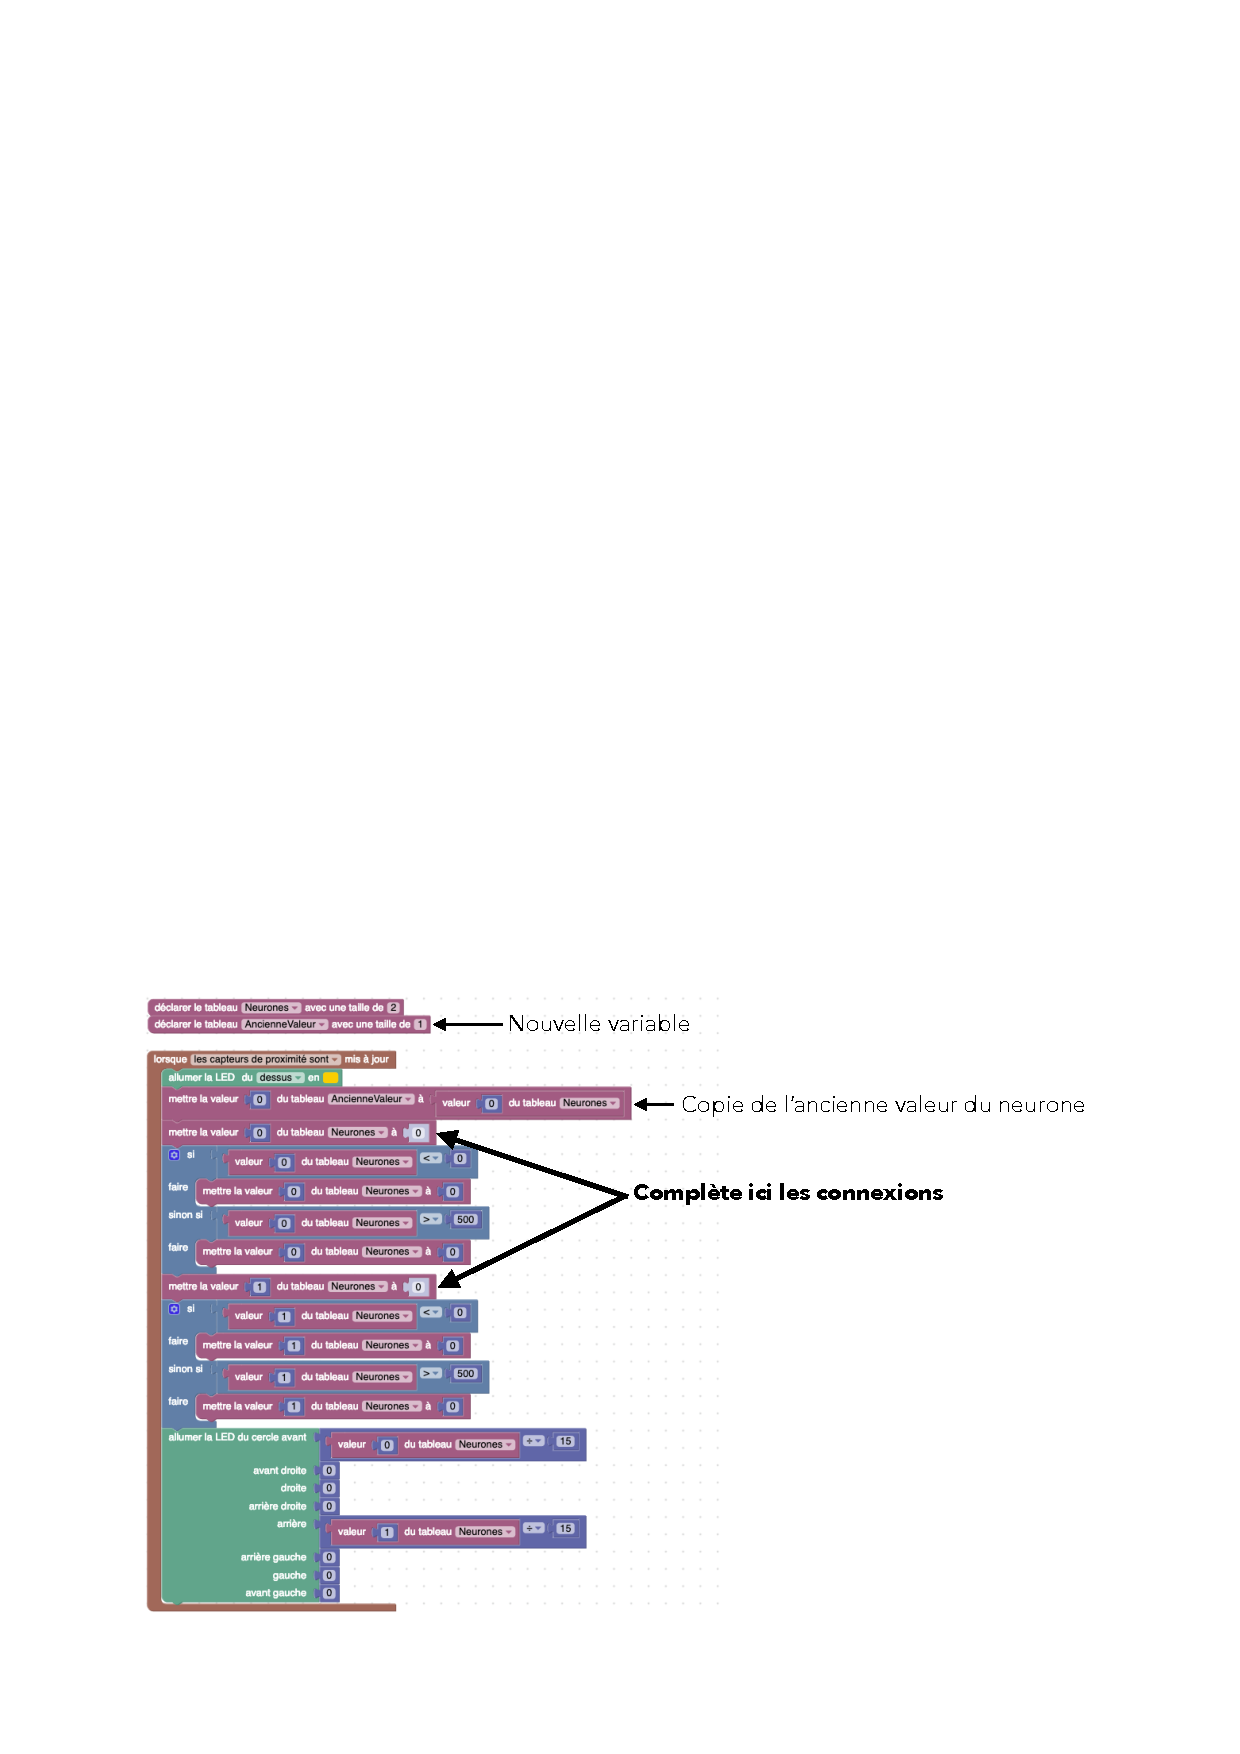
\includegraphics[width=\textwidth]{../ProgrammeEtape10.pdf}
\end{center}

\paragraph{Step 11:} Connect the output of one neuron to the left motor and the other neuron to the right motor. You should observe the robot move forward taking left and right steps.

\paragraph{Step 12:} 

Add inhibitory neurons from front-left and front-right sensors, like in step 7, to make the robot turn when it perceive an obstacle from one side or the other.

\begin{center}
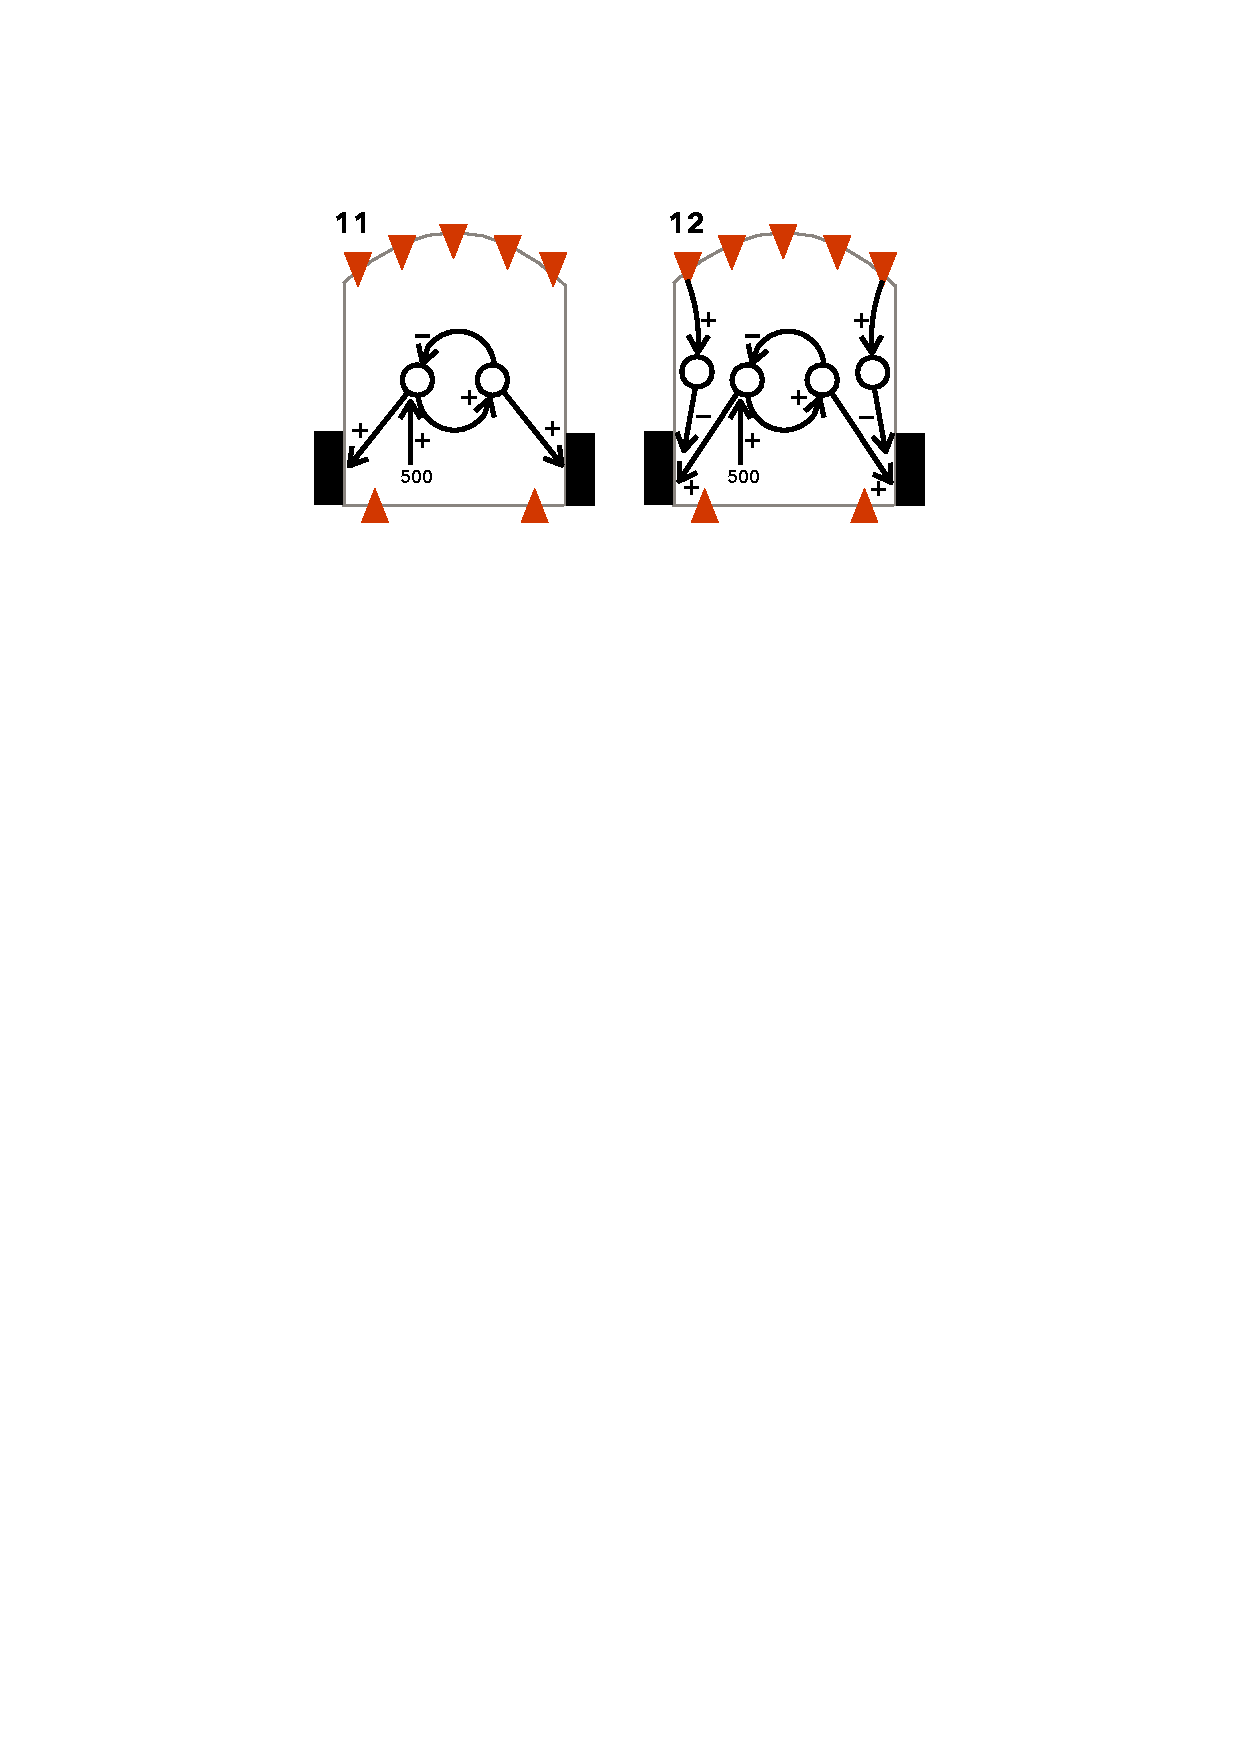
\includegraphics[width=0.66\textwidth]{../Etapes11-12.pdf}
\end{center}


\end{document}